\documentclass{nthuthesis}

% === Define Package
\usepackage{times}
\usepackage{verbatim}
\usepackage{color}
\usepackage{url}
\usepackage{graphicx}
\usepackage{array}
\usepackage{wallpaper}
\usepackage{cite}
\usepackage{physics}
\usepackage{multirow}
\usepackage{makecell}
\usepackage{hhline}
\usepackage{rotating}
\usepackage{amsmath}
\usepackage{tikz}
\usepackage{floatrow}
\usepackage{listings}
\usepackage{siunitx}
\usepackage{cleveref}
\usepackage{titlesec}
\usepackage{bm}
\usepackage{amssymb}
\usepackage{mathrsfs}
\usepackage{ragged2e}
\usepackage{indentfirst}
\usepackage{emptypage}
\usepackage{titletoc}
\usepackage{titlesec}
\usepackage{pdfpages}
\usepackage{notoccite} % PREVENTS CITES IN CAPTIONS FROM MISNUMBERING YOUR REFERENCES 
\usepackage{caption}
\usepackage[labelformat=simple]{subcaption} % Fig.1.1a >>>> Fig.1.1(a)
\renewcommand\thesubfigure{(\alph{subfigure})}
\usepackage[ruled,linesnumbered]{algorithm2e}

\titleformat{\section}
  {\normalfont\fontsize{18}{20}\bfseries}{\thesection}{1em}{}
\titleformat{\subsection}
  {\normalfont\fontsize{16}{20}\bfseries}{\thesubsection}{1em}{}

% Make caption format to be <Table,Figure> <Number> <Title>
\captionsetup[figure]{name={Figure },labelsep=space}
\captionsetup[table]{name={Table },labelsep=space}

\newcommand{\Paragraph}[1]{\paragraph{#1}\mbox{}\\} % New paragraph will add new line

\floatsetup[table]{capposition=top}

\makeatletter
% Reinsert missing \algbackskip
\def\algbackskip{\hskip-\ALG@thistlm}

\providecommand\add@text{}
\newcommand\tagaddtext[1]{%
  \gdef\add@text{#1\gdef\add@text{}}}% 
  
\renewcommand\tagform@[1]{%
  \maketag@@@{\llap{\add@text\quad}(\ignorespaces#1\unskip\@@italiccorr)}%
}

\makeatother

\newcommand{\Keywordsen}{\vspace*{\fill}\noindent\textbf{Keywords:}\ } % Keywords
\newcommand{\Keywordszh}{\vspace*{\fill}\noindent\textbf{關鍵字:}\ } % Keywords

% declare the path(s) where your graphic files are
\graphicspath{{./figsrc/}}
% and their extensions so you won't have to specify these with
% every instance of \includegraphics
% \DeclareGraphicsExtensions{.pdf,.jpeg,.png}

% Using the tex-text mapping for ligatures etc.
\defaultfontfeatures{Mapping=tex-text}

% Set the default fonts

% English font
% Note: please refer to 'fc-list :outline -f "%{family}\n"' for choosing a valid font name
\usepackage{fontspec}
%\setmainfont{Times New Roman.ttf}
\setmainfont{Times New Roman}

% Chinese font
% Note: please refer to 'fc-list :outline -f "%{family}\n"' for choosing a valid font name
\setCJKmainfont[AutoFakeBold=3,AutoFakeSlant=.4]{kaiu.ttf}
\setCJKmonofont[AutoFakeBold=3,AutoFakeSlant=.4]{kaiu.ttf}
\defaultCJKfontfeatures{AutoFakeBold=6,AutoFakeSlant=.4}

\CenterWallPaper{0.25}{nthulogo.png}


% Title Setting
\titleformat{\chapter}[display]
  {\Large\bfseries\centering}
  {\chaptertitlename\ \thechapter}{0pt}{\Large}
% \titleformat{\section}
%   {\sffamily\large\bfseries\centering}
%   {\thesection}{1em}{}
\titlespacing*{\chapter}{0pt}{0pt}{20pt}


% TOC setting
\titlecontents{chapter}% <section-type>
  [0pt]% <left>
  {\addvspace{1em}}% <above-code>
  {\bfseries\chaptername\ \thecontentslabel\quad}% <numbered-entry-format>
  {}% <numberless-entry-format>
  {\bfseries\hfill\contentspage}% <filler-page-format>

% Your information goes here
% author: Tz-Huan Huang [http://www.csie.ntu.edu.tw/~tzhuan]

% ----------------------------------------------------------------------------
% "THE CHOCOLATE-WARE LICENSE":
% Tz-Huan Huang wrote this file. As long as you retain this notice you
% can do whatever you want with this stuff. If we meet some day, and you think
% this stuff is worth it, you can buy me a chocolate in return Tz-Huan Huang
% ----------------------------------------------------------------------------

% Syntax: \var{English}{Chinese}
\university{National Tsing Hua University}{國立清華大學}
\college{College of Engineering
}{工學院}
\institute{Department of Power Mechanical Engineering}{動力機械工程學系碩士班}
\division{電控}
\title{A Research of Watering Gantry Robot in Greenhouse}{溫室用龍門型澆水機器人研究}
\author{Chi-Hao Lee}{李吉豪}
\studentid{108033532}
\advisor{Dr. Rongshun Chen}{陳榮順}
\defenseyear{2021}{一一O}
\defensemonth{December}{七}
\defenseday{30}


\begin{document}

\frontmatter

\makecover
% \makecopyright


% 電子檔著作權授權書
% 紙本論文著作權授權書
% 電子檔案上網授權書
% 延後公開申請書
% 指導教授推薦書
% 考試委員審定書

\makeatletter\@twosidefalse\@mparswitchfalse\makeatother

\begin{abstractzh}
\setcounter{page}{1}
植物的良好生長與澆水量之適當呈正相關,而植物的疾病發生與葉面的濕度有高度相關。在現代農業的溫室栽培,植株澆灌水量與方位之精確的控制可以降低疾病。以往主要的澆灌方式,一為人工持噴罐頭灑水,二為自溫室頂部灑水,然而比較此兩種方式,前者需要耗費人力且水量不精確,而後者雖然簡單方便,卻會造成葉面浸潤,進而增加植物的疾病發生率,且仍然無法精確控制個別植株的水量。

本研究研發一新型多制動龍門型澆水機器人,可應用於蝴蝶蘭植株栽培溫室中。首先藉由應用YOLOv4-tiny物件辨識技術,偵測植株位置,再經由計算圖像回歸直線以估測植株姿態。並且利用反應變形路徑演算法進行路徑規劃,以降低姿態估測的不確定性。最後透過控制龍門上的噴水頭位置制動器,使制動器沿著規劃路徑移動,藉以避開葉面區域澆水,最終減少葉面之潮濕度。

本研究建構於機器人系統(ROS)上,並且透過Nvidia Xavier實現演算法。最終,與過往的研究比較,本研究實現了82\%的澆水成功率,根據使用者設定,可以達到每秒3個植株以上的速度進行精準澆水。

\end{abstractzh}


\begin{abstracten}
The growth of the plants is positively correlated to the amount of watering. Also, the incidence rate is often highly related to the humidity of the leaves. In modern greenhouse agriculture, the precise control of watering direction and amount can reduce the incident rate of plants. In the past, there were two primary watering ways for the greenhouse: The first one is manual watering that requires human resources and cannot precisely control the water direction and amount. The other one is the overhead irrigation system, which is convenient and straightforward but will cause infiltration on the leaf surface, increasing the incidence rate of plants and fail to control the water amount on each plant.

This research develops a new type of gantry robot to water Phalaenopsis orchid seedlings in the greenhouse. First, this work uses YOLOv4-tiny as the neural network model to locate the seedlings and to regress the cropped image to estimate the poses of the seedlings. Furthermore, the reactive deformation trajectory planning algorithm is utilized to generate the sprayer trajectory and to reduce the uncertainty of pose estimation. Finally, multiple sprayers are guided along the planned path to water the soil portion other than the leaf area of plants, which can mitigate the infiltration on leaves.

The gantry robot is implemented on the robot operation system (ROS) that runs on an Nvidia Xavier computer. Eventually, compared with the earlier works, the proposed system guarantees that the watering success rate and the watering speed can reach 82\% and at least three seedlings per second, respectively.
\end{abstracten}

\begin{comment}
    \keywords{Object detection, Path planning, Gantry robot, Computer vision, Orchids, Greenhouse, Smart farming, Robot Operation System}
\end{comment}

%\begin{comment}
%\category{I2.10}{Computing Methodologies}{Artificial Intelligence --
%Vision and Scene Understanding} \category{H5.3}{Information
%Systems}{Information Interfaces and Presentation (HCI) -- Web-based
%Interaction.}
%
%\terms{Design, Human factors, Performance.}
%
%\keywords{Motor control, Path planning, Smart agriculture}
%\end{comment}
\begin{acknowledgementsen}
\setcounter{page}{0}

我要感謝R欠~~~~~~

\end{acknowledgementsen}

{\singlespacing
\tableofcontents
\listoffigures
\listoftables
}

\mainmatter

\makeatletter\@twosidetrue\@mparswitchtrue\makeatother

% Your thesis goes here
\chapter{Introduction}
\label{c:introduction}

\section{Overview}
\label{section:overview}

This research aims to develop a novel gantry machine to precisely water the soil portion of orchid seedlings, the incidence rate of which will be accordingly decreased due to lower infiltration on leaves. In the previous research of Cartesian watering machines, the entire performance was decreased because of the high time cost to turn the watering valve on and off. It is supposed that the seedling grows symmetrically with two sides of leaves aligned on a straight line. This research installs the watering sprayers on the motion actuators, which are controlled to pass through the seedlings center perpendicular to the leaves' growth direction in order to prevent splashing water from leaves. Three main topics in this research are:

\begin{enumerate}
    \item Pose estimation of 2D Seedling
    \item Trajectory planning of gantry actuator
    \item Prototype implementation of gantry robot 
\end{enumerate}

The seedling pose estimator provides the seedling position and the growth direction of leaves using YOLOv4-tiny and regression of the region of interest (RoI). Then, the trajectory planner will control the linear actuators using the pose of seedlings. Finally, this research completes the prototype of the gantry machine, entitled ``XsY gantry robot'', to implement the proposed methods. Unlike the XY gantry machine, which has a single coordinate system, the XsY gantry robot is a multi-coordinate system that shares the same y-axis. Therefore, the name ``XsY'' means that the robot has multiple x-axes that are controllable, as shown in Fig.\ref{fig:xsymodel}.

\begin{figure}[ht]
    \centering
    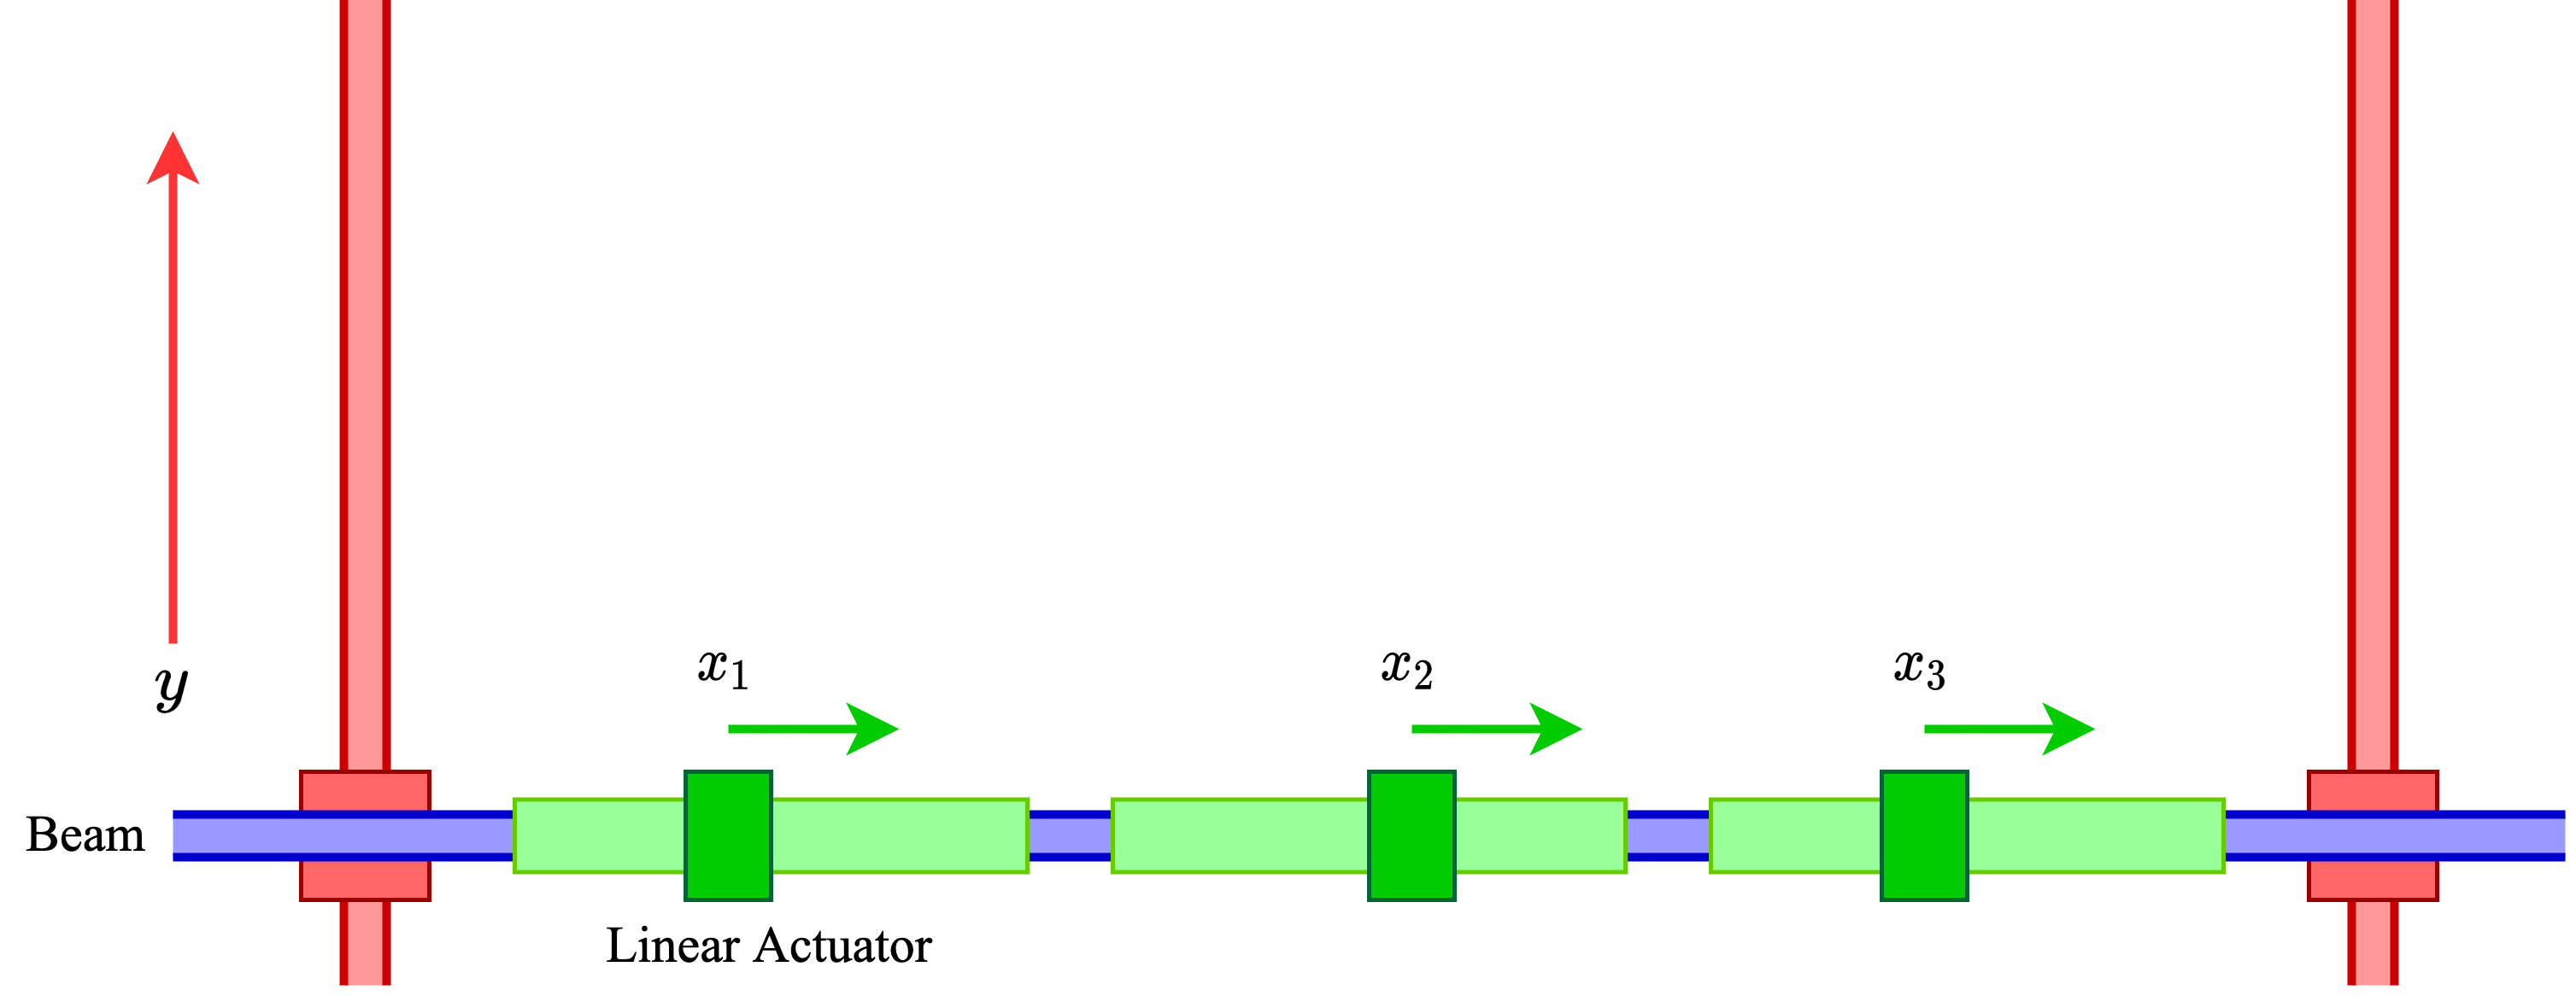
\includegraphics[width=0.7\textwidth]{figsrc/ch01/XsY Gantry.png}
    \caption{XsY gantry model}
    \label{fig:xsymodel}
\end{figure}


To evaluate the performance of this work, two metrics are adopted to determine the performance of the gantry robot: watering success rate and watering speed.

% ===== Check Line V2 2021/08/09
% ===== Check Line V2.1 2021/08/24

\section{Background and Motivation}
\label{section:motivation}

% The importance of agriculture in Taiwan
From the 1960s, Taiwan began to develop floriculture for the purpose of industrial diversification. However, in recent years, Taiwan has encountered severe structural problems: the rapid aging of the agricultural population and the scarcity of young farmers entering the profession. The lack of agricultural population, a significant problem, currently impacts the agriculture of Taiwan, particularly in floriculture. According to the statistical data from The Council of Agriculture in Taiwan\cite{行政院農委會_農業就業人口統計}, the agricultural population was only 550 thousand until March 2020. Furthermore, these farmers' average age is highly old at 62 in 2017\cite{黃柏軒_2018} and will be much older in the future. Due to this challenge, it is an essential mission for Taiwan to develop intelligent and automatic agriculture.

% Orchids
Moreover, as an important plant with a high economic value in Taiwan, the number of orchids reaches up to 15.8 million USD, out of 78\% of the overall exportation of flowers, with exports. In addition, the phalaenopsis (or moth orchids), one of the species of orchids, has even an exporting value of more than 13.9 million USD, 88\% of the total orchids, as shown in Fig.\ref{fig:export-orchid}\cite{行政院農委會_單一農產品進出口量值}.

\begin{figure}[ht]
    \centering
    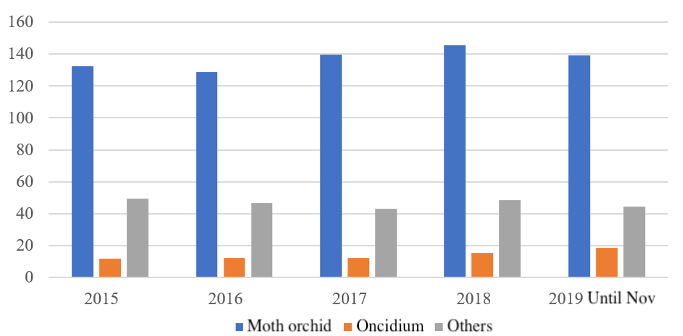
\includegraphics[width=0.8\textwidth]{ch01/export_orchid_en.png}
    \caption{Exporting Value of Orchids In Past Years In Taiwan}
    \label{fig:export-orchid}
\end{figure}

% Automatic system
In the modern greenhouse, companies tend to introduce various automatic systems rather than human power to automate the production process, which can help solve the laboring shortage of agriculture. In most situations, the automatic machine can enhance the product quality and curtail the laboring cost. However, it is still advantageous for humans to tackle some sophisticated tasks. Especially in agriculture, the irregular shapes of plants make it difficult to be treated by machine. Furthermore, despite being designed for automatic watering, seeding, or pollination, earlier research works may only focus on specific species. In this research, the main problem comes from the usage of the watering machine.

% The watering
The watering system plays a critical role in the manufacture of orchids. Plants need to be watered to grow and live; simultaneously, farmers mix the fertilizer and the water to make it easier for plants to absorb the nutrient. Originally, most of the watering tasks are completed by the human. For example, Fig.\ref{fig:HumanWater} demonstrates that the farmer uses a water jet to water the orchid seedlings.

\begin{figure}[ht]
    \centering
    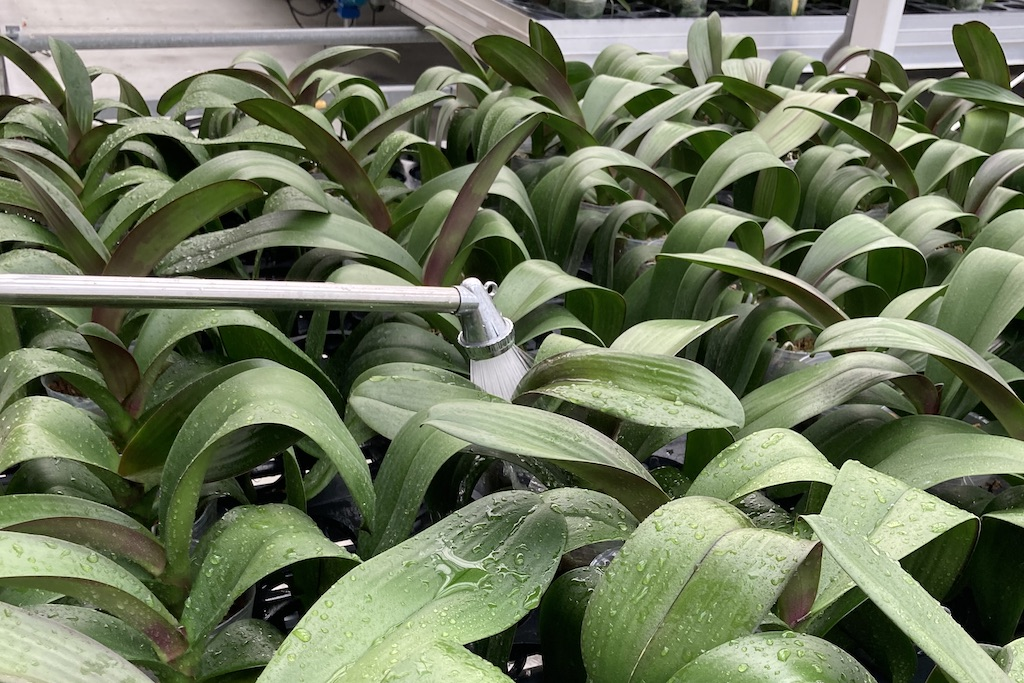
\includegraphics[width=0.7\textwidth]{ch01/HumanWater.jpeg}
    \caption{Farmer is Watering Using Water Jet}
    \label{fig:HumanWater}
\end{figure}

% ===== Check Line V2 2021/08/03

% Using overhead irrigation sys
Recently, most greenhouse companies adopt multiple types of watering machines to solve the lack of laboring resources, including the overhead irrigation system, as shown in Fig.\ref{fig:irrigation_sprinkler}. The overhead irrigation system is cheaper than other systems due to its simple design. Most of the cost comes from the installation of pipes. Besides, by adjusting the inlet valve, the amount of water to plants is controllable. For example, a computer controls the valve to water the whole greenhouse in our cooperative company periodically.

% overhead irrigation sys disadvantage, using gantry
However, the overhead irrigation system will make the whole greenhouse moist, leading to more plant diseases. According to the research about plant diseases from A. Henn, C. Hong and G. Moorman\cite{henn_2016, Plant_Pathogens}, the incidence rate of plants increases with the moisture in the air or the water on leaves. Facing this problem, the cooperative orchid greenhouse has tried another approach, such as the simple watering gantry machine showed in Fig.\ref{fig:old_gantry}. The watering gantry machine is fixed, and there is a set of water sprayers on it. The machine can water plants on the planting bed uniformly by pushing the planting bed and by spreading the water from the water spray. This solution keeps water spread under the gantry so that it decreases the moisture inside the greenhouse.

\begin{figure}[ht]
    \centering
    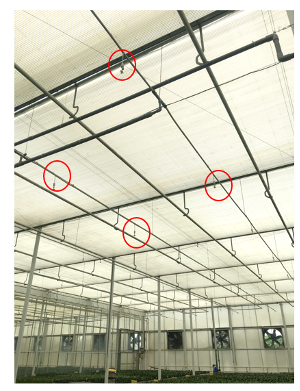
\includegraphics[height=6cm]{ch01/irrigation_sprinkler_1.png}
    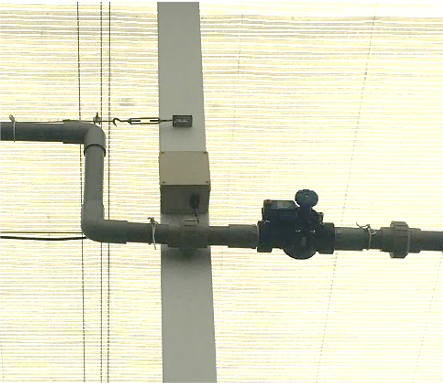
\includegraphics[height=6cm]{ch01/irrigation_sprinkler_2.png}
    \caption{Overhead Irrigation System Installed in Greenhouse}
    \label{fig:irrigation_sprinkler}
\end{figure}

% gantry disadvantage
In spite of preventing the increment of moisture in the greenhouse, the watering gantry machine still suffers some problems. For example, the sprayers installed on the device remain watering both plant roots and leaves. The excessive water accumulation in the root consequently causes the death of plants. Besides, after using the gantry machine, the infiltration on leaves is still not solved, which also increases the incidence rate of plants.

\begin{figure}[ht]
    \centering
    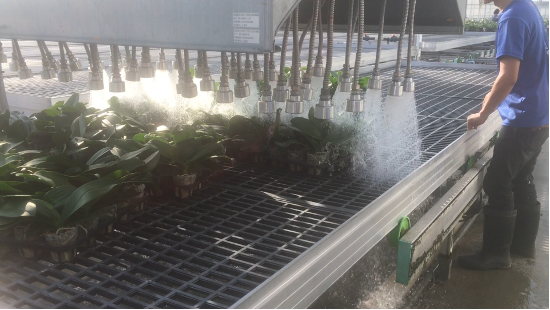
\includegraphics[height=6cm]{ch01/old_gantry_1.png}
    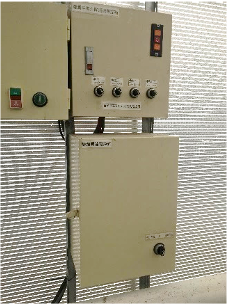
\includegraphics[height=6cm]{ch01/old_gantry_2.png}
    \caption{Traditional Gantry Water Machine}
    \label{fig:old_gantry}
\end{figure}

Until now, a large number of automatic machines cannot solve the difficult problem that a large amount of water remains on the leaves after the orchid seedlings are watered. Additionally, it is not reasonable to avoid the disadvantages of the watering machine by instead adopting human power in large-scale farming. Thus, in recent years, the techniques of computer vision and neural networks have been developed to help resolve many agricultural problems, such as using a convolutional neural network to count the number of seedlings\cite{jausih_2020}. Furthermore, there are also researches of agricultural robots trying to build an automatic system to monitor and control the growth of plants individually. Hence, the research of agricultural robots may be a practical solution to the remaining water problem.
% \input{02_methodology}
% \input{03_Implementation}
% \input{04_result-and-discussion}
% \input{05_conclusion}

\appendix

\backmatter

\renewcommand{\bibname}{References}
\addcontentsline{toc}{chapter}{\bibname}
\bibliographystyle{ieeetr}

% Your bibliography goes here
{\singlespacing
 \bibliography{thesis}
}

\appendix
\chapter*{Appendix}
\label{c:appendix}

Appendix

\end{document}
